\renewcommand{\arraystretch}{0.1}% Tighter
\centering \footnotesize
\begin{tikzpicture}
\node[] (start) {};
\node[left=1cm of start] (sfsigma) {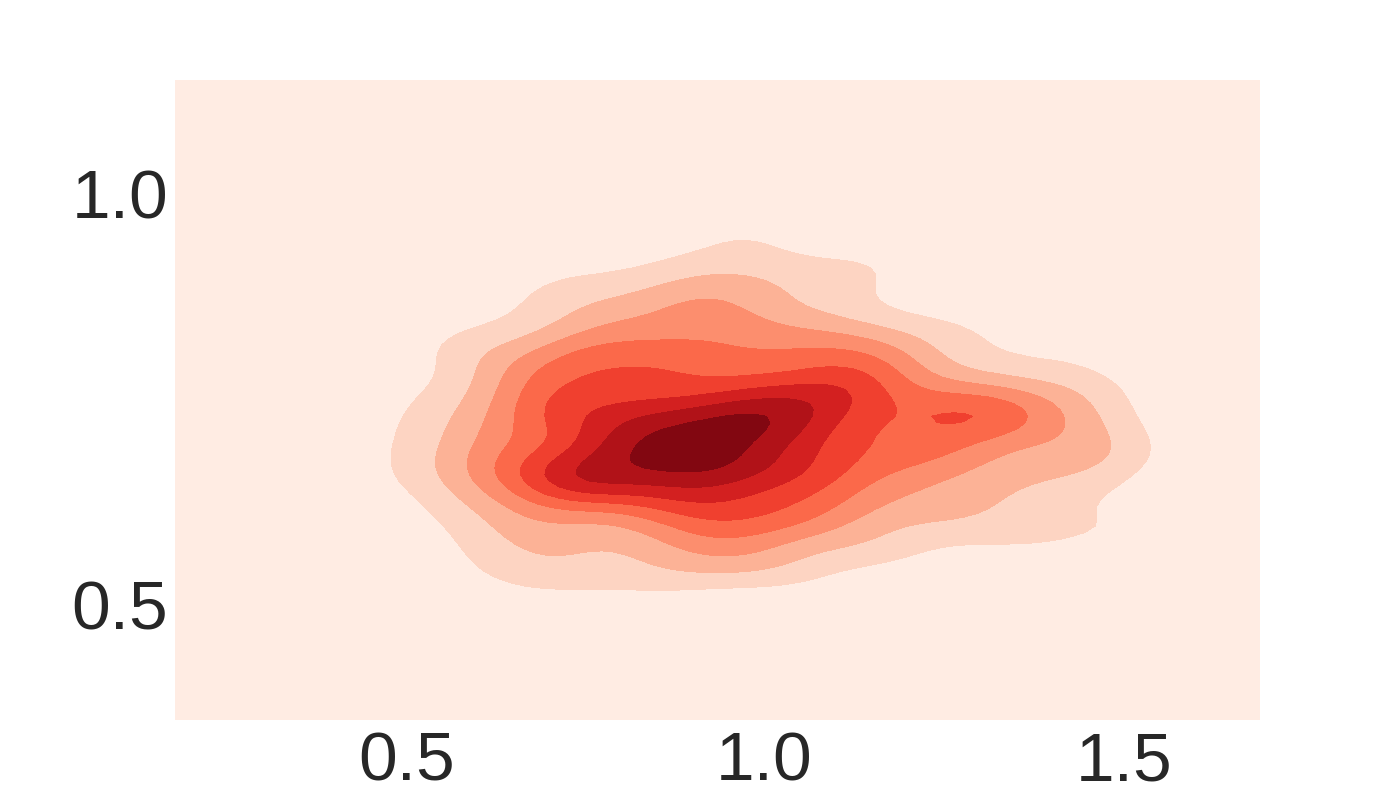
\includegraphics[height=2cm]{figs/hypers_sf_sigma.png}};
\node[right=1cm of start] (sfell) {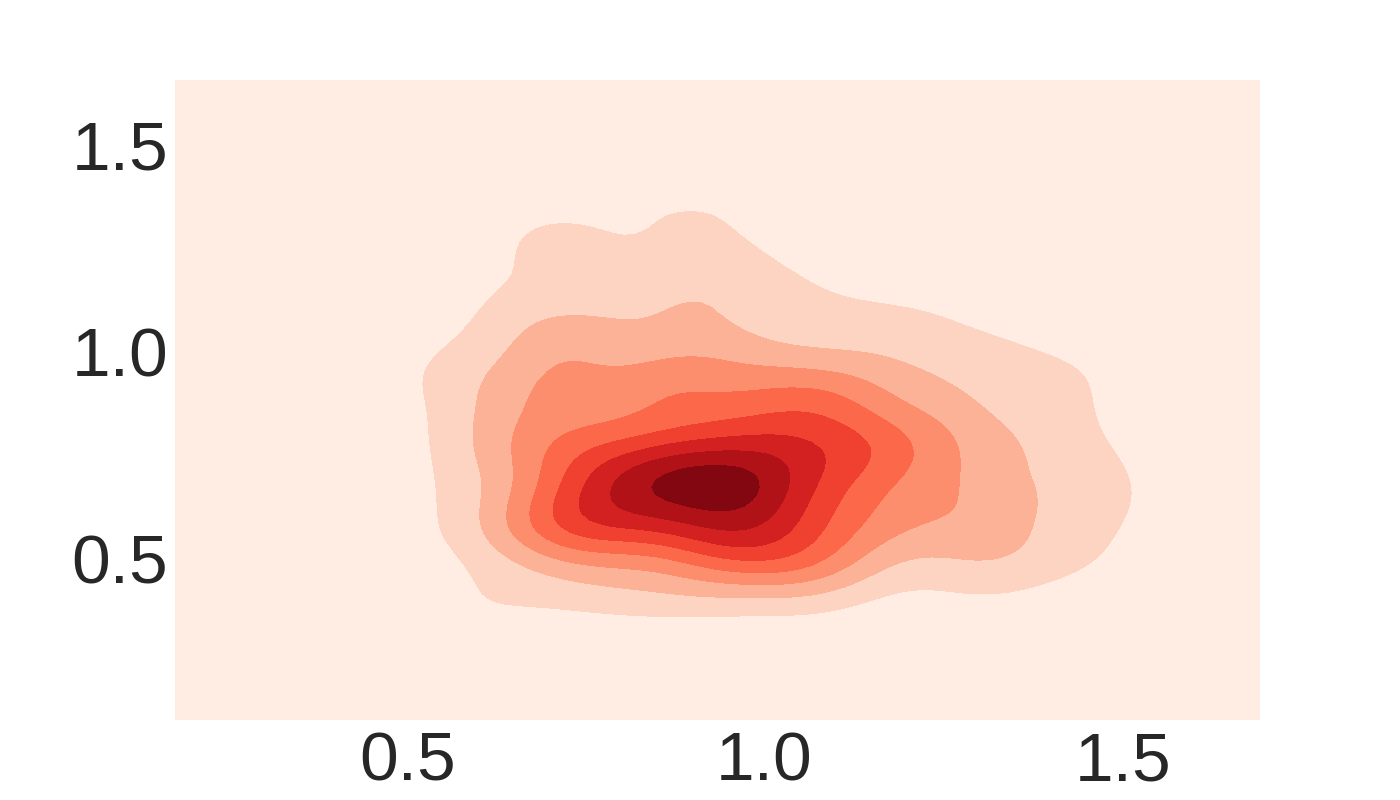
\includegraphics[height=2cm]{figs/hypers_sf_ell.png}};
\node[above=1cm of start] (hyper) {(a) $P(\bm{\theta} = \{\ell,sf,\sigma\} \mid \mathbf{D,K})$};
\node[left=0.cm of sfsigma] (ell) {$\ell$};
\node[below=0.cm of sfsigma] (sf1) {$sf$};
\node[left=0.cm of sfell] (sigma) {$\sigma$};
\node[below=0.cm of sfell] (sf2) {$sf$};
\end{tikzpicture}
\begin{tabular}{ll} \hline
\multicolumn{2}{}{}
  \begin{minipage}{4cm}
 \footnotesize\begin{lstlisting}
 // Data and look-up function
 define data = array(array(-1.87, 0.13), ..., array(1.67, 0.81))
 assume f_look_up = proc(index) {lookup(data, index)}
\end{lstlisting}
\end{minipage}\\
\hline
\multicolumn{2}{}{}
  \begin{minipage}{4cm}
 \footnotesize\begin{lstlisting}
 assume sf = tag("hyper", 0, gamma(alpha_sf, beta_sf)))
 assume l = tag("hyper", 1, gamma(alpha_l, beta_l)))
 assume sigma = tag("hyper", 2, uniform_continuous(0, 2))
\end{lstlisting}
\end{minipage}
  \\
\hline
\footnotesize\begin{lstlisting}[ belowcaptionskip=0.1\baselineskip,mathescape,escapechar=\#]
// The covariance function
assume se = make_squaredexp(sf, l)
assume wn = make_whitenoise(sigma)
assume composite_covariance = add_funcs(se, wn)#\vspace{1mm}#
// Create a prober and emulator using gpmem
assume (f_compute, f_emu) =
    gpmem(f_look_up, composite_covariance)#\vspace{1mm}#
sample f_emu(array(-2, $\cdots$, 2))
\end{lstlisting}
 &  \raisebox{-0.5\height}{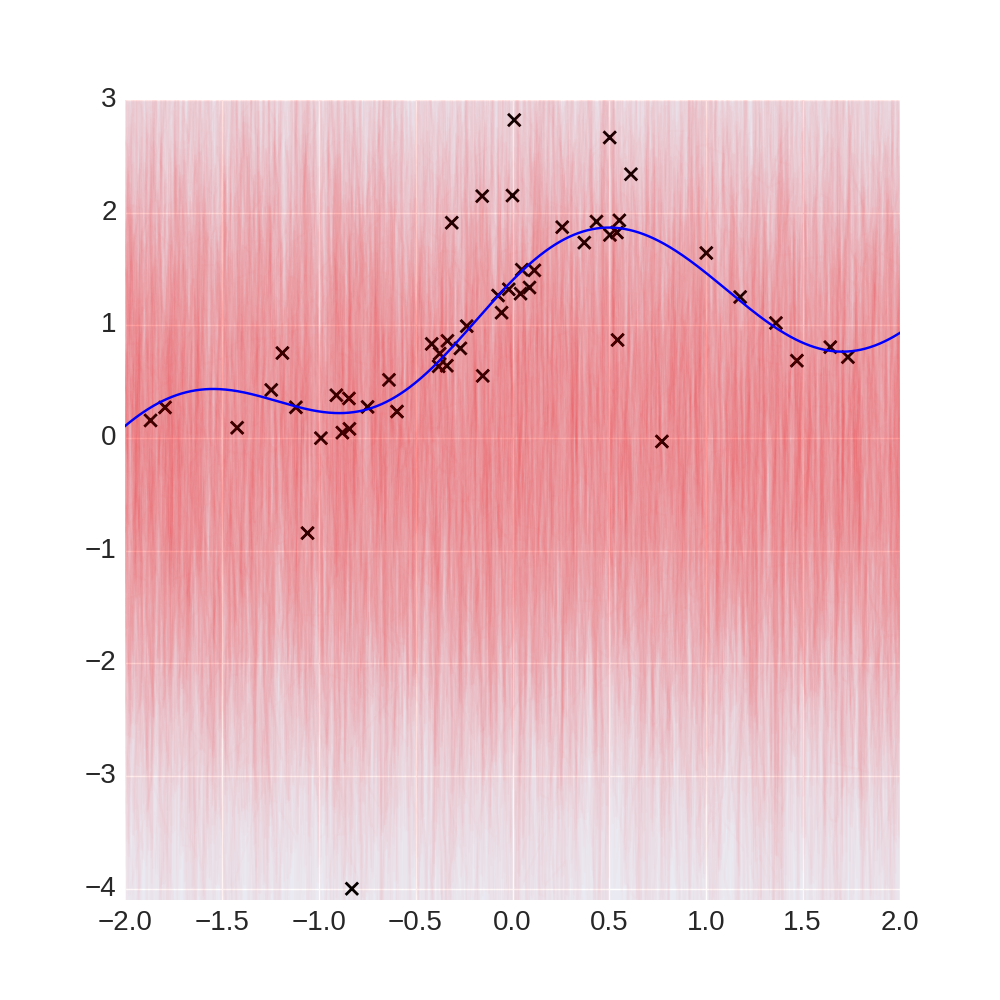
\includegraphics[height=3.4cm]{figs/neal_example_before_observation.png}}  \\ \hline
% line 3

\footnotesize\begin{lstlisting}[aboveskip=-0.8 \baselineskip,mathescape,escapechar=\#]
// Observe all data points
for n ... N
    observe f_emu(first(lookup(data,n))) =
        second(lookup(data,n))
// Or: probe all data points
for n ... N
    predict f_compute(first(lookup(data,n)))#\vspace{1mm}#
sample f_emu(array(-2, $\cdots$, 2))
\end{lstlisting}
 &  \raisebox{-0.5\height}{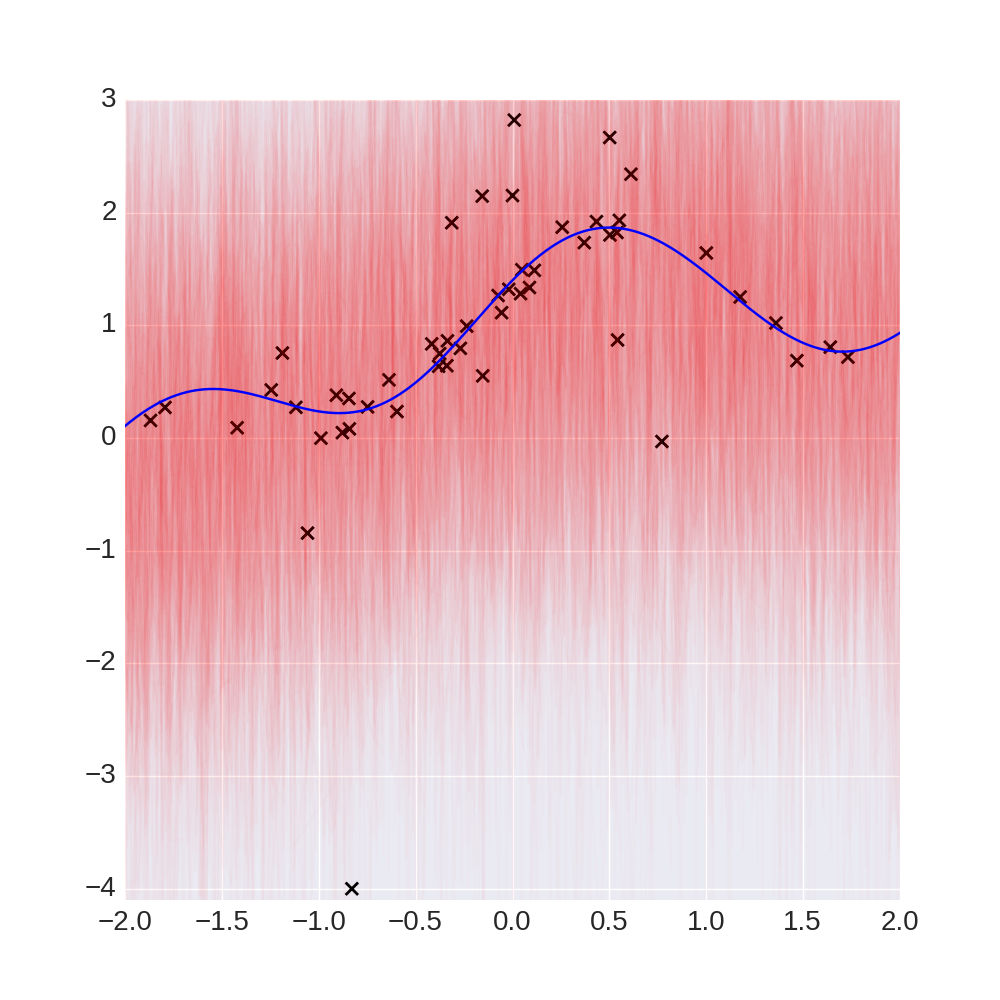
\includegraphics[height=3.4cm]{figs/neal_example_after_observation.png}}  \\ \hline
\footnotesize\begin{lstlisting}[mathescape,escapechar=\#]
// Metropolis-Hastings
infer repeat(100, do(
    mh("hyperhyper", one, 2),
    mh("hyper",      one, 1)))#\vspace{1mm}#
sample f_emu(array(-2, $\cdots$, 2))
\end{lstlisting}
 &   \raisebox{-0.5\height}{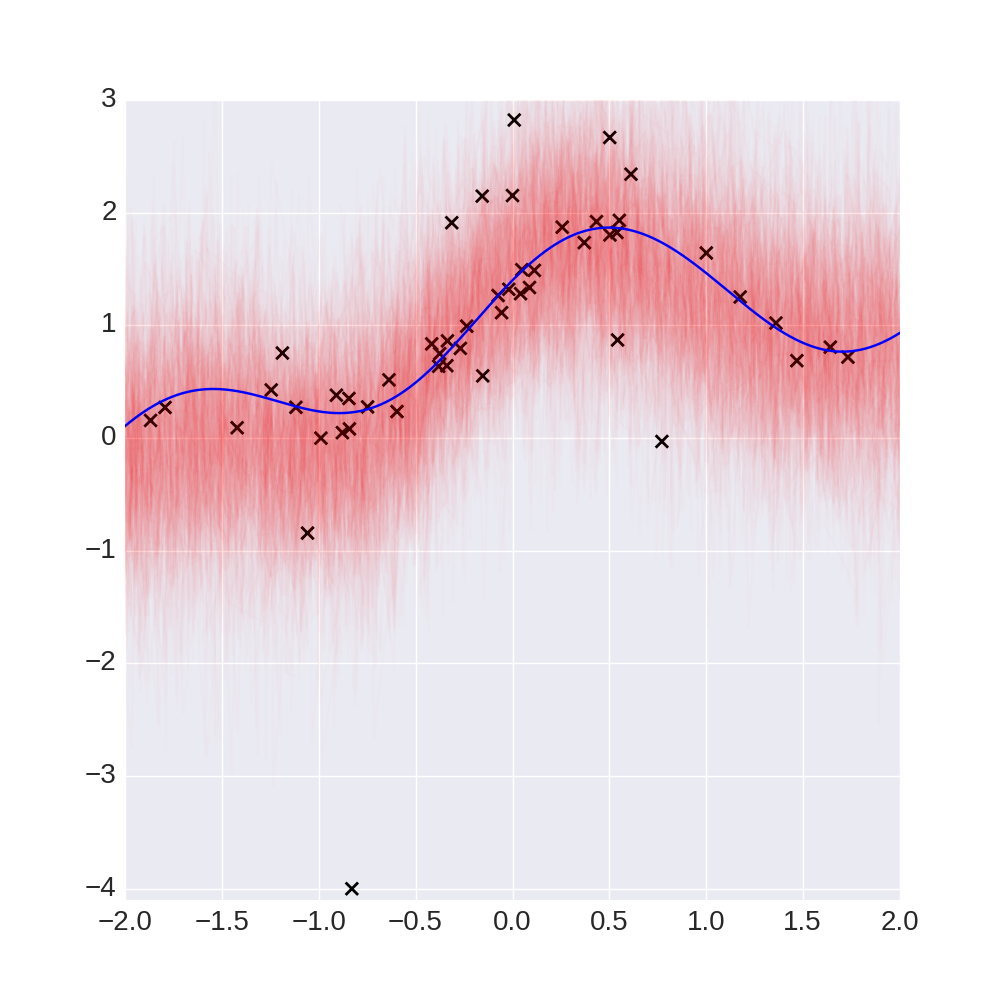
\includegraphics[height=3.4cm]{figs/neal_Bayesian.png}} \\ \hline
\footnotesize\begin{lstlisting}[mathescape,escapechar=\#]
// Optimization
infer map("hyper", all, 0.01, 15)

sample f_emu(array(-2, $\cdots$, 2))
\end{lstlisting}
 &   \raisebox{-0.5\height}{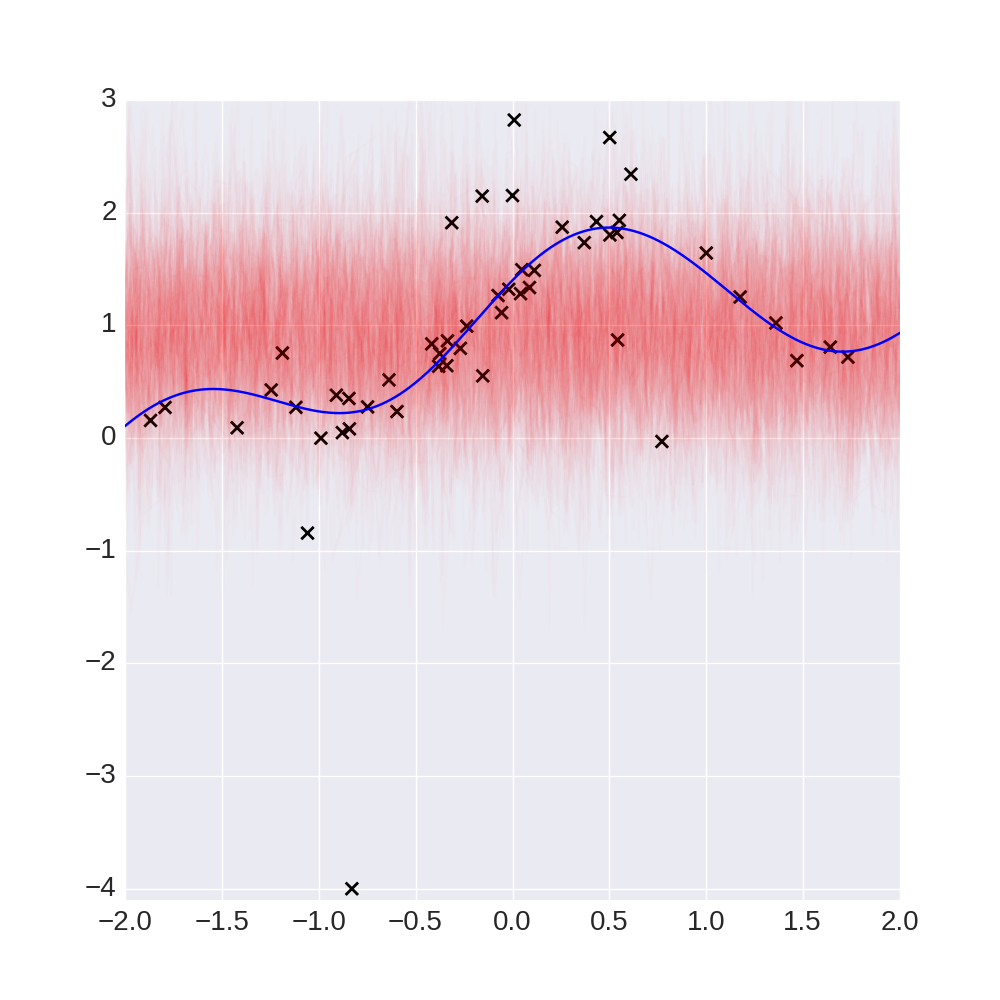
\includegraphics[height=3.4cm]{figs/neal_example_map_inference_alpha0p01_iter15.png}} \\ \hline

 \end{tabular}
